\documentclass[10pt,letterpaper]{article}
\usepackage{tools}
\usepackage{enumitem}
%\settextfont{B Nazanin}
\usepackage{lipsum}
\setlength{\parskip}{3mm}
\setlength{\parindent}{0mm}
\newcommand{\wid}{0.49\textwidth}
\newcommand{\widone}{60mm}
\begin{document}
\Large
\begin{center}
In the name of beauty

5th problem set solution of ComNet course
\hl
\end{center}
Q1)
\begin{enumerate}[label=\alph*-]
\item
True. The rdt 3.0 protocol is a special case of both of GBN- and SR protocol without pipelining (window size = 1).
\item
False. The same problem encountering in SR protocol when choosing the window size and max. seqnum arbitrarily could also arise in GBN protocol.
\item
False. Since the receiver behaves differently in the protocols, so must the sender to adapt itself to the difference.
\item
False. TCP connection is full-duplex which makes it desirable for two-way, secure connections
\item
False (but slightly!). Also the second segment cannot carry any payload, since the first two segments are dedicated for connection setup (not that addressed in the Networl Layer!)
\end{enumerate}

Q2) Recall the TCP connection is full-duplex and therefore established in both the directions. In this scheme, both sender and receiver choose an initial seqnum arbitrarily in $[0,499]$, which is announced to the other side of the transmission via ACK segments. A packet with seqnum=289 is considered as legit only if it matches any of the allowed sequence numbers in the sender. This can happen only if the receiver has chosen the initial seqnum from $\{39,289\}$. Hence the probability of failure becomes ${2\over 500}=0.004$ and the probability of correct performance becomes $0.996$.

Q3) 
%Assume a sender transmits 4 segments back-to-back labeled from 0 to 3 to a receiver:
%\newpage
%\begin{figure}[htb]
%\centering
%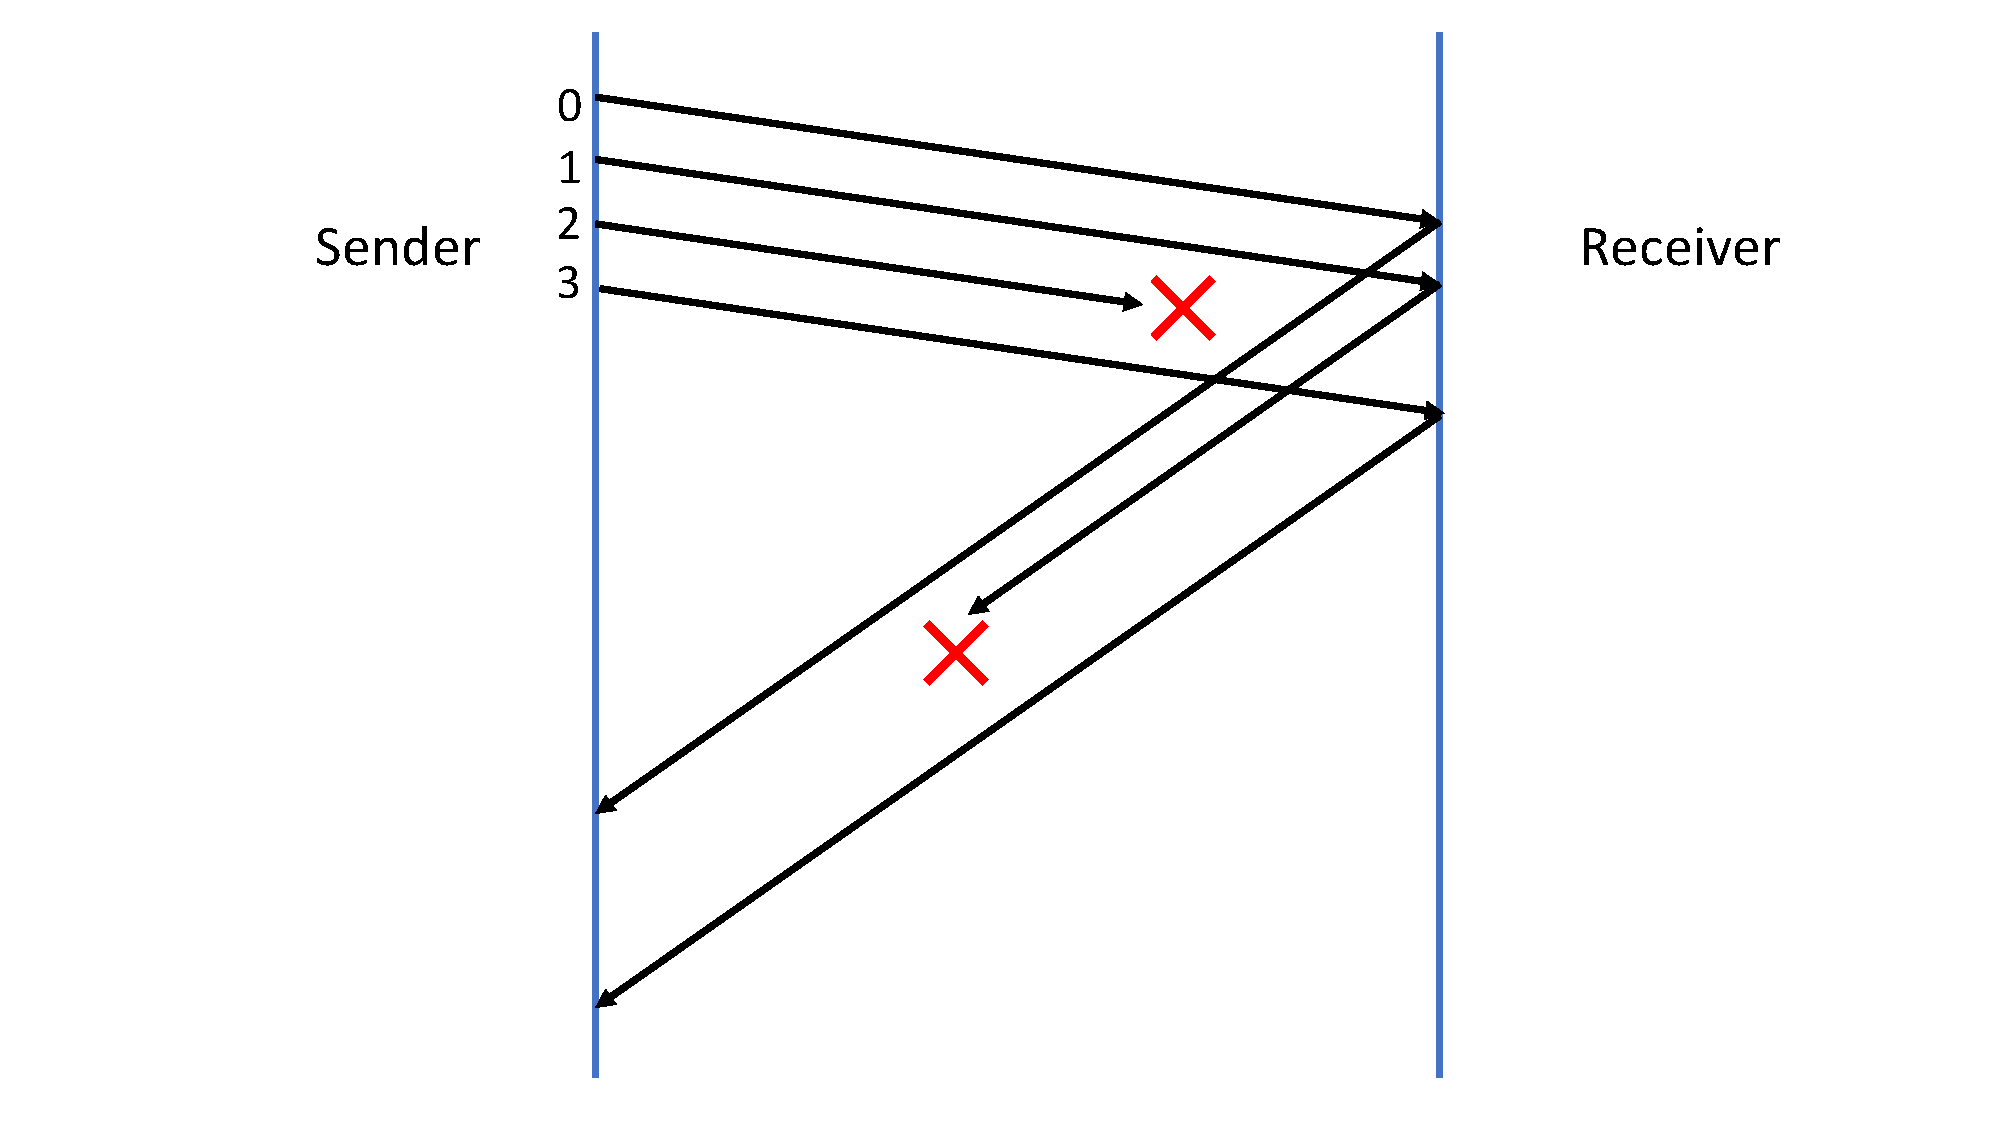
\includegraphics[width=100mm]{gbn_sr.pdf}
%\caption{rdt2.1 sender}
%\end{figure}
The packet numbered 2 does not make it all the way to the receiver and the packet numbered 1, is correctly received but the corresponding ACK does not reach the sender. Describe what operations would SR and GBN perform.

The packet with seqnum=0 is received correctly and successfully ACKed, hence the window would move on from it and will take care of packets with seqnum$\ge1$.
\begin{itemize}
\item
GBN:
\begin{enumerate}
\item
The receiver would send two ACKs for packet 1 (once on packet 1 reception and once after dropping packet 3).
\item
Either the sender retransmits packets \{1,2,3\} due to TIMEOUT or it receives the ACK for packet 1, so that it pushes its window to be started from packet 2 and retransmits packets \{2,3\}.
%Sender would retransmit the packets \{2,3\} after its TIMEOUT for them is raised sequentially (not simultaneously). 
\item
The procedure above repeates itself until all the packets are received and ACKed correctly.
\end{enumerate}
\item
SR:
\begin{enumerate}
\item
The receiver would send two ACKs for packets \{1,3\}.
\item
The sender would retransmit any packet when the corresponding TIMEOUT for it is alerted.
%Sender would retransmit the packets \{2,3\} after its TIMEOUT for them is raised sequentially (not simultaneously). 
\item
The procedure above repeates itself until all the packets are received and ACKed correctly.
\end{enumerate}
\end{itemize}

Q4) Let us denote the probability that the i-th packet is successfully delivered to the receiver by $\Pr\{X_i=k\}$. The i-th packet is received correctly in a single transmission only if all of its predecessor packets (i.e. those numbered from 0 to $i-1$) have been successfully received, which has a probability of, say, $q_i$. Since each packet has a probability of $1-p$ to undergo the channel, we obtain:
$$
q_i=(1-p)^{i+1}
$$
and the $k$-th correct reception follows a geometric distribution such as
\[
\begin{split}
\Pr\{X_i=k\}&=
%\Pr\{X_i=k|\text{All previous packets received correctly up to }k\}
%\\&\times
%\Pr\{\text{All previous packets received correctly up to }k\}
%\\&+
%\Pr\{X_i=k|\text{!(All previous packets received correctly up to }k)\}
%\\&\times
%\Pr\{!\text{(All previous packets received correctly up to }k)\}
%\\&=
(1-q_i)^{k-1}q_i
\end{split}
\]
with the following mean:
$$
n_i={1\over q_i}={1\over (1-p)^{i+1}}
$$
%Determine the following statements as true or false with enough reasons.
%\begin{enumerate}[label=\alph*-]
%\item
%Both trasport and network layer protocols provide logical communication between processes running at different hosts rather than hosts themselves.
%\item
%Transport layer packets are refered to as \textbf{datagrams}.
%\item
%TCP ensures that the transmitted packets would finally reach their destination, however it makes no guarantee on the order of packets.
%\item
%The IP service model is a best-effort delivery service since it guarantees to deliver segments between communicating hosts, whether orderless or not.
%%\item
%%Cookies are used to keep track of user IDs in a stateless HTTP server.
%%\item
%%Link-layer switches are typically capable of processing the packets up to the layer 3.
%%\item
%%SMTP and FTP are examples of layer 1 protocols while TCP is a transport layer protocol.
%%\item
%%API is a set of rules 
%%\item
%%For economical reasons, exploiting optical fibers is not recommended in long-haul network
%\end{enumerate}
%
%Q2)
%\begin{enumerate}[label=\alph*-]
%\item
%Why is IP said to be an unreliable service and if so, how would TCP provide reliable data transfer on top of IP?
%\item
%Why are source and destination host port numbers included in segment headers? What problem could arise if they are ignored?
%\end{enumerate}
%
%Q3) Suppose Client A initiates a Telnet session with Server S. At about the same
%time, Client B also initiates a Telnet session with Server S. Provide possible
%source and destination port numbers for
%\begin{enumerate}[label=\alph*-]
%\item
%The segments sent from A to S.
%\item
%The segments sent from B to S.
%\item
%The segments sent from S to A.
%\item
%The segments sent from S to B.
%\item
%If A and B are different hosts, is it possible that the source port number in
%the segments from A to S is the same as that from B to S?
%\item
%How about if they are the same host?
%\end{enumerate}
%(Choose the port numbers at source and destination arbitrarily.)
%
%Q4) Consider the following Figure. What are the source and destination port values in the segments
%flowing from the server back to the clients’ processes? What are the IP
%addresses in the network-layer datagrams carrying the transport-layer segments?
%\begin{figure}[ht]
%\centering
%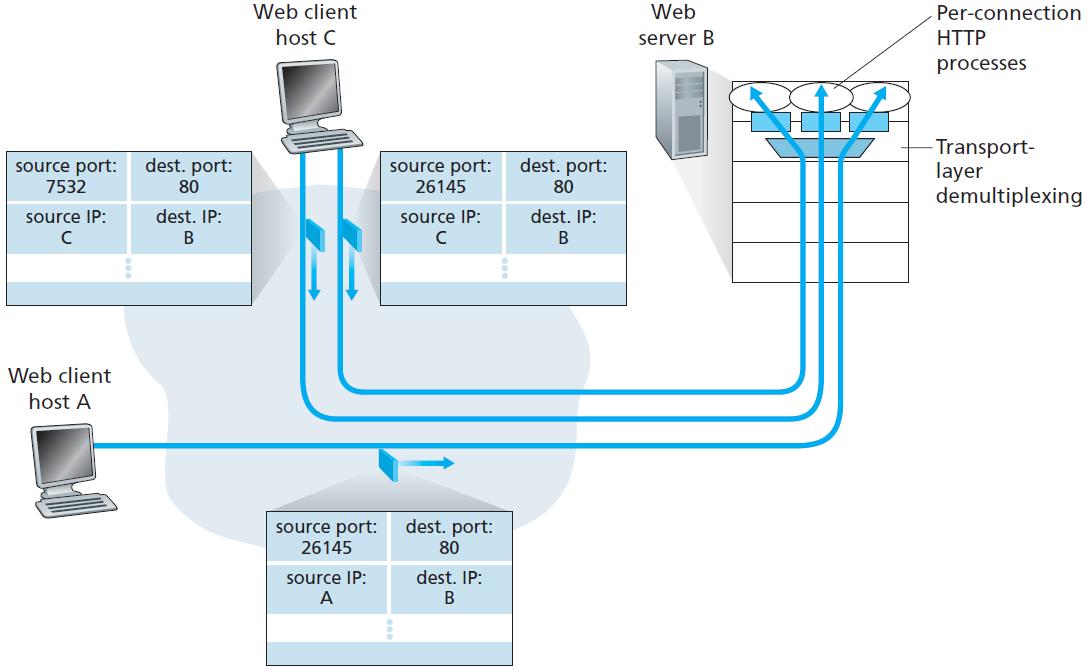
\includegraphics[width=180mm]{simnet}
%\end{figure}
\end{document}